\documentclass[crop,tikz]{standalone}
\usetikzlibrary{backgrounds}
\colorlet{blue}{cyan}
\tikzset{
  inverted/.style = {
    color=white,
    background rectangle/.style={fill},
    show background rectangle
  }
}

\usetikzlibrary{calc,positioning,shapes}

\begin{document}
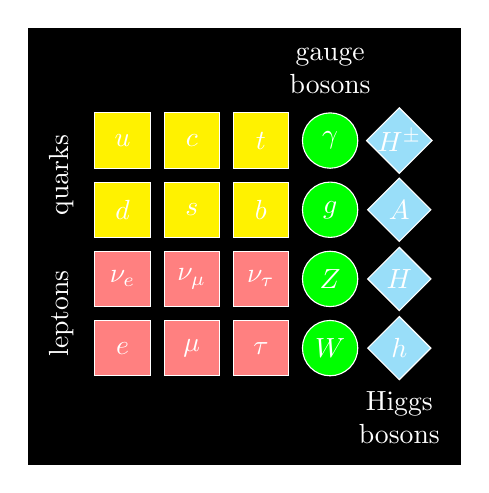
\begin{tikzpicture}[inverted,
  node distance = 2.5em,
  quark/.style  = {rectangle, white, draw, fill=yellow , minimum width=2em  , text centered, minimum height=2em  , inner sep=0pt},
  lepton/.style = {rectangle, white, draw, fill=red!50 , minimum width=2em  , text centered, minimum height=2em  , inner sep=0pt},
  gauge/.style  = {circle   , white, draw, fill=green  , minimum size=2em   , text centered, minimum height=2em  , inner sep=0pt},
  scalar/.style = {diamond  , white, draw, fill=blue!40, minimum width=2.3em, text centered, minimum height=2.3em, inner sep=0pt},
  ]
  \node[quark] (u) {$u$};
  \node[quark, below of=u] (d) {$d$};
  \node[quark, right of=u] (c) {$c$};
  \node[quark, below of=c] (s) {$s$};
  \node[quark, right of=c] (t) {$t$};
  \node[quark, below of=t] (b) {$b$};
  \node[lepton, below of=d] (ne) {$\nu_e$};
  \node[lepton, below of=ne] (e) {$e$};
  \node[lepton, right of=ne] (nm) {$\nu_\mu$};
  \node[lepton, below of=nm] (m) {$\mu$};
  \node[lepton, right of=nm] (nt) {$\nu_\tau$};
  \node[lepton, below of=nt] (ta) {$\tau$};
  \node[gauge, right of=t] (gamma) {$\gamma$};
  \node[gauge, below of=gamma] (g) {$g$};
  \node[gauge, below of=g] (Z) {$Z$};
  \node[gauge, below of=Z] (W) {$W$};
  \node[scalar, right of=W] (h) {$h$};
  \node[scalar, above of=h] (H) {$H$};
  \node[scalar, above of=H] (A) {$A$};
  \node[scalar, above of=A] (Hp) {$H^\pm$};
  % labels
  \node[rotate=90,above] (quarks)  at ($(u)!0.5!(d)+(-0.5,0)$)  {quarks};
  \node[rotate=90,above] (leptons) at ($(ne)!0.5!(e)+(-0.5,0)$) {leptons};
  \node[below of=h, align=center] (higgs) {Higgs\\ bosons};
  \node[above of=gamma, align=center] (gauge) {gauge\\ bosons};
\end{tikzpicture}
\end{document}
